% \documentclass[a4paper,biblatex, 10pt]{jacow}
\documentclass[twocolumn,DIV=14,a4paper,biblatex, 10pt]{scrartcl}
% \usepackage{polyglossia}
\usepackage{biblatex}
\usepackage{microtype}
\usepackage{crimson}
\usepackage{hyperref}
\usepackage{xspace}
\usepackage{tikz}
\usetikzlibrary{patterns}
\usetikzlibrary{plotmarks}
\usetikzlibrary{intersections}
% \usepackage{newtxmath}

\usepackage{lipsum}
\usepackage{graphicx}
\usepackage{siunitx}

\usepackage{ifthen}
\newboolean{uprightparticles}
\setboolean{uprightparticles}{true}
%\input{lhcb-symbols-def.tex}

\addbibresource{bib.bib}
% \setdefaultlanguage{english}


\newcommand{\atlaspix}{\texttt{ATLASpix1}\xspace}
\newcommand{\timepix}{\texttt{Timepix3}\xspace}
\newcommand{\tot}{\texttt{ToT}\xspace}
\newcommand{\corry}{\texttt{Corryvreckan}\xspace}
\newcommand{\ROOT}{\texttt{ROOT}\xspace}


\title{F96 - Characterisation of Silicon Pixel Sensors for High-Energy Physics and beyond}
\author{Robin Heinemann, Jonas Reichert, University Heidelberg, Heidelberg, Germany}
\date{July 2020}

\begin{document}

\maketitle

\begin{abstract}
  \lipsum[1]
\end{abstract}

\section{Introduction}
Silicon pixel sensors are widely used in particle physics to detect, track and analyse ionizing particles. They work by measuring the current pulse in a reverse biased diode that is produced by the charge carriers drifing to the electrodes when a ionizing particle hits the depletion region and produces new electron-hole pairs. The number fo charge carriers produced depends on on the energy of the ionizing particle so the energy of the ionizing particle can be measured by measuring the area of the current pulse. By placing many diodes in a 2D array, the location can be determined and by measuring the time the current pulse initially crosses the threshold (time of arrival - \texttt{ToA}) the time.
In practice this is done by measuring the time the current is above a certain threshold, the time-over-threshold (\tot), see figure~\ref{fig:tot}.

\begin{figure}
  \begin{center}
    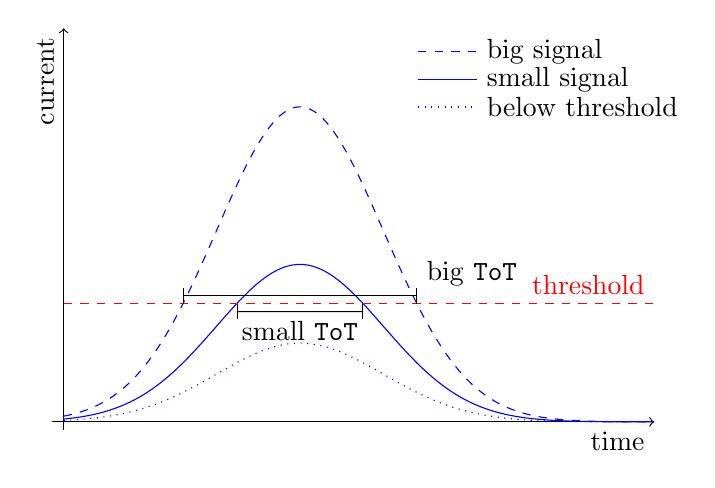
\begin{tikzpicture}[xscale=1.5]
      \draw[->] (-0.1,0) -- (5, 0) node[below left]{time};
      \draw[->] (0,-0.1) -- (0, 5) node[above left,rotate=90]{current};
      \draw[blue,dotted,domain=-2:3, samples=400] (0, 0) plot ({\x + 2},{exp(-\x*\x)});
      \draw[blue,domain=-2:3,samples=400,name path=small] (0, 0) plot ({\x + 2},{2*exp(-\x*\x)});
      \draw[blue,dashed,domain=-2:3, samples=400,name path=big] (0, 0) plot ({\x + 2},{4*exp(-\x*\x)});
      \draw[red,dashed,name path=thres] (0, 1.5) -- ++(5, 0) node[above left] {threshold};
      \draw[|-|,name intersections={of={small and thres},by={A,B}}] ([yshift=-0.1cm]A) -- node[midway,below] {small \tot} ([yshift=-0.1cm]B);
      \draw[|-|,yshift=0.5,name intersections={of={big and thres},by={A,B}}] ([yshift=0.1cm]A) -- ([yshift=0.1cm]B) node[above right,align=right] {big \tot};
      \draw[blue, dotted] (3.0, 4) -- ++(0.5,0) node[black,right,align=left] {below threshold};
      \draw[blue] (3.0, 4.35) -- ++(0.5,0) node[black,right,align=left] {small signal};
      \draw[blue, dashed] (3.0, 4.7) -- ++(0.5,0) node[black,right,align=left] {big signal};
    \end{tikzpicture}
  \end{center}
  \caption{Time-over-threshold measurement illustration\label{fig:tot}}
\end{figure}

The classical design for silicon pixel sensors are \textbf{hybrid pixel sensors}. Here the diodes are on a seperate chip from the readout part. Usually they are connected by bump-bonding. The \timepix sensors used in the reference telescope for this analysis are of this kind.

A alternative are monolythic active pixel sensors (\texttt{MAPS}), that combine detection diode and readout logic on the same chip. In the \texttt{HVMAPS} variant an additional high voltage on the order of $\SI{100}{\volt}$ is applied as reverse bias.

In the following we will analyse the spatial and temporal resolution and accuracy of the \atlaspix sensor, a new \texttt{HVMAPS} sensor.
\section{Setup}
We analyse the \atlaspix sensor using the test-beam facility at the Super-Proton Synchrotron (\texttt{SPS}) at \texttt{CERN}. It provides a beam of charged pions with a momentum of $\SI{120}{\giga\electronvolt}$. The data we are analysing is from run $\num{29663}$ taken in November 2018. In this run, the bias voltage was set to $\SI{-75}{\volt}$, the threshold voltage to $\SI{750}{\milli\volt}$ and a clock period of $\SI{8}{\nano\second}$ was used.

To analyse the \atlaspix sensor a reference telescope of \timepix sensors is used to determine the actual track of each particle, which is then compared to the data measured by the \atlaspix. The \atlaspix sensor (DUT) is placed inbetween the \timepix sensors and the \timepix sensors are tilted slightly to increase the chance of a particle hitting multiple pixels, which can be used to increase the spatial resolution. Figure \ref{fig:detector_setup} shows a schematic drawing of the measurement setup.

\begin{figure*}
  \begin{center}
    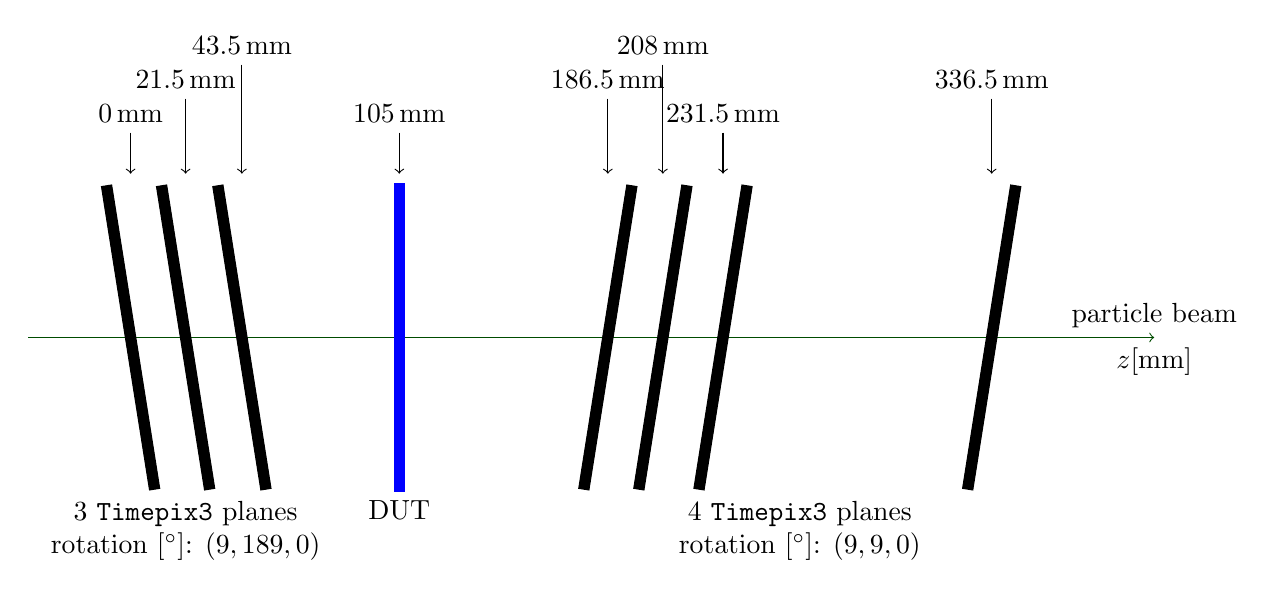
\begin{tikzpicture}
      \begin{scope}[scale=1.3]
        \draw[color=green!30!black, ->] (-1,0) -- ++(11, 0) node[above,color=black] {particle beam} node[below,color=black] {$z [\si{\milli\meter}]$};

        \node[below] (DUT) at (105.0/ 40, -1.5) {DUT};
        \node[below, align=center] (timepix1) at (21.5/ 40, -1.5) {3 \timepix planes\\rotation [$\si{\degree}$]: $(9, 189, 0)$};
        \node[below, align=center] (timepix2) at (186.5/ 80 + 336.5/80, -1.5) {4 \timepix planes\\rotation [$\si{\degree}$]: $(9, 9, 0)$};

        \foreach[count=\i] \x/\rx/\ry/\c in {0/9/9/black, 21.5/9/9/black, 43.5/9/9/black, 105/0/0/blue, 186.5/-9/9/black, 208/-9/9/black, 231.5/-9/9/black, 336.5/-9/9/black}{
          \filldraw[color=\c, rotate around={\rx:(\x / 40,0)}] (\x / 40 - 0.05, -1.5) rectangle ++(0.1, 3);
          \draw[->] (\x / 40, {1.5 + Mod(\i + 2, 3) / 3 + 0.5}) node[above] {$\SI{\x}{\milli\meter}$} -- (\x / 40, 1.6);
        }
      \end{scope}
    \end{tikzpicture}
  \end{center}
  \caption{Schematic of detector setup\label{fig:detector_setup}}
\end{figure*}

\section{Analysis}
To analyse the \atlaspix the general idea is to first reconstruct the track taken by a particle using the reference \timepix sensors and then compare the track with the position and time measured by the \atlaspix sensor. These steps are carried out using \corry\cite{corry} and \ROOT\cite{root}.

% Particle physics experiments need detectors to observe the particles produced in a collision. To get better results a new generation of pixel detectors is needed. Pixel detectors are based on semiconductor technology and mainly made from silicon. Current detectors are hybrid detectors, which have two separate units for the detection of a particle hit and the readout.Those parts need to be connected by wires or bump bonds, which limit spatial resolution and scalability.

% A new class of detectors is under test. Monolithic detectors combine the detection and readout in a single chip. One of them is the \atlaspix, the device under test (DUT) in this experiment. It was originally developed for the ATLAS inner tracking system (ITk) at the LHC. The design implements the comparator inside the pixel cell to avoid long transmission length of the analogous signal at the cost of a larger pixel capacitance arising from the comparator logic.

% The data used in this analysis was recorded during the run 29663 in November 2018 by the CLICdp collaboration at CERN. The DUT was operated with a bias of $\SI{-75}{\volt}$, a threshold of $\SI{750}{\milli\volt}$ and a clock period of $\SI{8}{\nano\second}$.


The silicon pixel sensors are based on pn-junctures, which are operated in reverse bias. This is a diode. The pn-junctures consists of a p-type semiconductor, which has excess positive charges and a n-type semiconductor, which has excess negative charges. At the contact surface of the two semiconductors, the  charge gradient give rise to an diffusion current, which drives the recombination of the charges. This area is called the depletion zone, which features only very few free charges. The depletion zone is dominated by the ionised atomic trunks, which have a negative charge for the n-type semiconductor and a positive charge for the p-type semiconductor. These difference gives rise to a drift current in opposite direction of the diffusion current. The electric field in the depletion zone is linearly growing. For the depth of the depletion zone in the p-type semiconductor $x_p$ and in the n-type semiconductor $x_n$, the electric field takes the form
$$E (x) = \left\{
\begin{array}{ll}
\frac{-e N_A}{\epsilon \epsilon_0}(x_p+x) & -x_p<x<0 \\
\frac{e N_A}{\epsilon \epsilon_0}((x-x_n) & 0<x<x_n \\
\end{array}
\right. $$
with the permittivity $\epsilon$ of the material. The voltage over the depletion zone can be calculated from the difference in the potential between the two borders of the depletion zone. The potential in the depletion zone is
$$\phi (x) = \left\{
\begin{array}{ll}
\phi_p+\frac{-e N_A}{2\epsilon \epsilon_0}(x_p+x)^2 & -x_p<x<0 \\
\phi_n+\frac{e N_A}{2\epsilon \epsilon_0}((x-x_n)^2 & 0<x<x_n \\
\end{array}
\right. $$
where $\phi_p$ and $\phi_n$ are the potentials at $-x_p$ and $x_n$ respectively. Using the relations of the intrinsic Fermi-energy $E_f$ and extrinsic Fermi-energies $E_F$, we find the relations
$$E_f-E_F^p=-\phi_p=kT\ln{\frac{N_A}{n_i}}$$
$$E_f-E_F^n=-\phi_n=kT\ln{\frac{N_D}{n_i}}$$
This yields the voltage over the depletion zone
$$U_b=\frac{kT}{e}\ln{\frac{N_A N_D}{n_i^2}}$$
We can find this voltage also as a function of the depths of the depletion zone in the two materials,
$$U_b = \int_{x_p}^{x_n}E(x)dx=\frac{e}{e\epsilon \epsilon_0}x_p^2 \frac{N_A}{N_D}(N_A+N_D)$$
We can estimate the fraction of the depths as $\frac{x_n}{x_p}\approx \frac{N_A}{N_D}$ and see that the depletion zone is mainly expressed in the part with the lower doping.\\
If we now introduce an external voltage over the depletion zone, the system is no longer in thermal equilibrium and we have a concentration of $np >n_i^2$ and $np<n_i^2$ respectively. If the external voltage is positive on the p-type side, the voltage over the depletion zone decreases and the drift current becomes smaller than the diffusion current. Therefore the depletion zone becomes smaller. If the voltage is negative on the p-type side, however, the reverse effect takes place and the depletion zone becomes larger. As the depletion zone is the area in which particles are detected, it is the latter mode in which the detector diode is operated.\\
High energetic particles deploy their energy in the material and can create charges through ionisation. 


\section{Data processing}
The data is processed using the analysis program \texttt{Corryvreckan}. The used data was taken during the run 29663 in November 2018 by CLICdp. The data is analyzed in slices of $\SI{20}{\micro\second}$ to reduce the requirements on the RAM.

In a first step the data is imported using the modules 'EventLoaderTimepix' and 'EventloaderATLASpix'. Subsequently the 'Clustering4D' module is applied to find cluster, which arise from on a particle hitting multiple pixels of a detector or from charge spilling over. These clusters are assigned the position of their ToT-weight center of gravity and in addition the pixel in the cluster with the highest ToT is named the seed pixel.

In the next step the module 'Corrrelations' is applied to receive plots of the spatial correlation of the detectors relative to the reference detector. This is used to do a first correction of the alignment. This is done by the module 'Prealignment', which determines the peak of the correlations and updates the geometry file in a way that the peaks are shifted to zero.

Then the module 'Tracking4D' is applied which reconstructs the trajectory of the particle by searching for hits on a ellipsoid on the planes along the estimated tracks. This allows then to group the signals one particle produces along his track. Based on this result a precise alignment for the telescope planes is calculated by the module 'AlignmentTrackChi2'. It iterative alters the position and rotation of the telescope planes and refits the tracks trying to minimize the $\chi^2$ value.

Based on the telescope alignment the tracks on the DUT are reconstructed by the module 'DUT Association'. Using this results the DUT can finally be precisely aligned by the module 'AlignmentDUTResiduals', which iterative alters the DUTs translation and rotation trying the minimize the absolute of the Residuals.

The telescope and the DUT data is now sufficiently calibrated and the full data set analyzed. In addition the full analysis is run again for a grid of altering values of x and y spatial cuts in order to determine the dependence of the pixel efficiency from these factors. The spatial cuts give the distance which a hit can differ from the supposed position and is still considered belonging to the track.

To improve the time resolution of the sensor, the timewalk effect can be corrected by the module \texttt{AnalysisTimingATLASpix}. The timewalk effect refers to the dependence of the delay between hit and detection on the signals size. 

\section{Results}
We used the aligned data set to investigate the properties of the  \atlaspix sensor with respect to the reference sensor. 

We find the time resolution of the sensor by fitting a Gaussian function on the central parts of the time residual distribution shown in Fig. \ref{fig:time_residuals}. For this we used the interval between $\SI{-130}{\nano\second}$ and $\SI{-90}{\nano\second}$. The offset of the peak is depending on the system and not relevant for our analysis. We find the time resolution

\begin{equation}
  \Delta t = \SI{14.06}{\nano\second}
\end{equation}

\begin{figure}
  \centering
  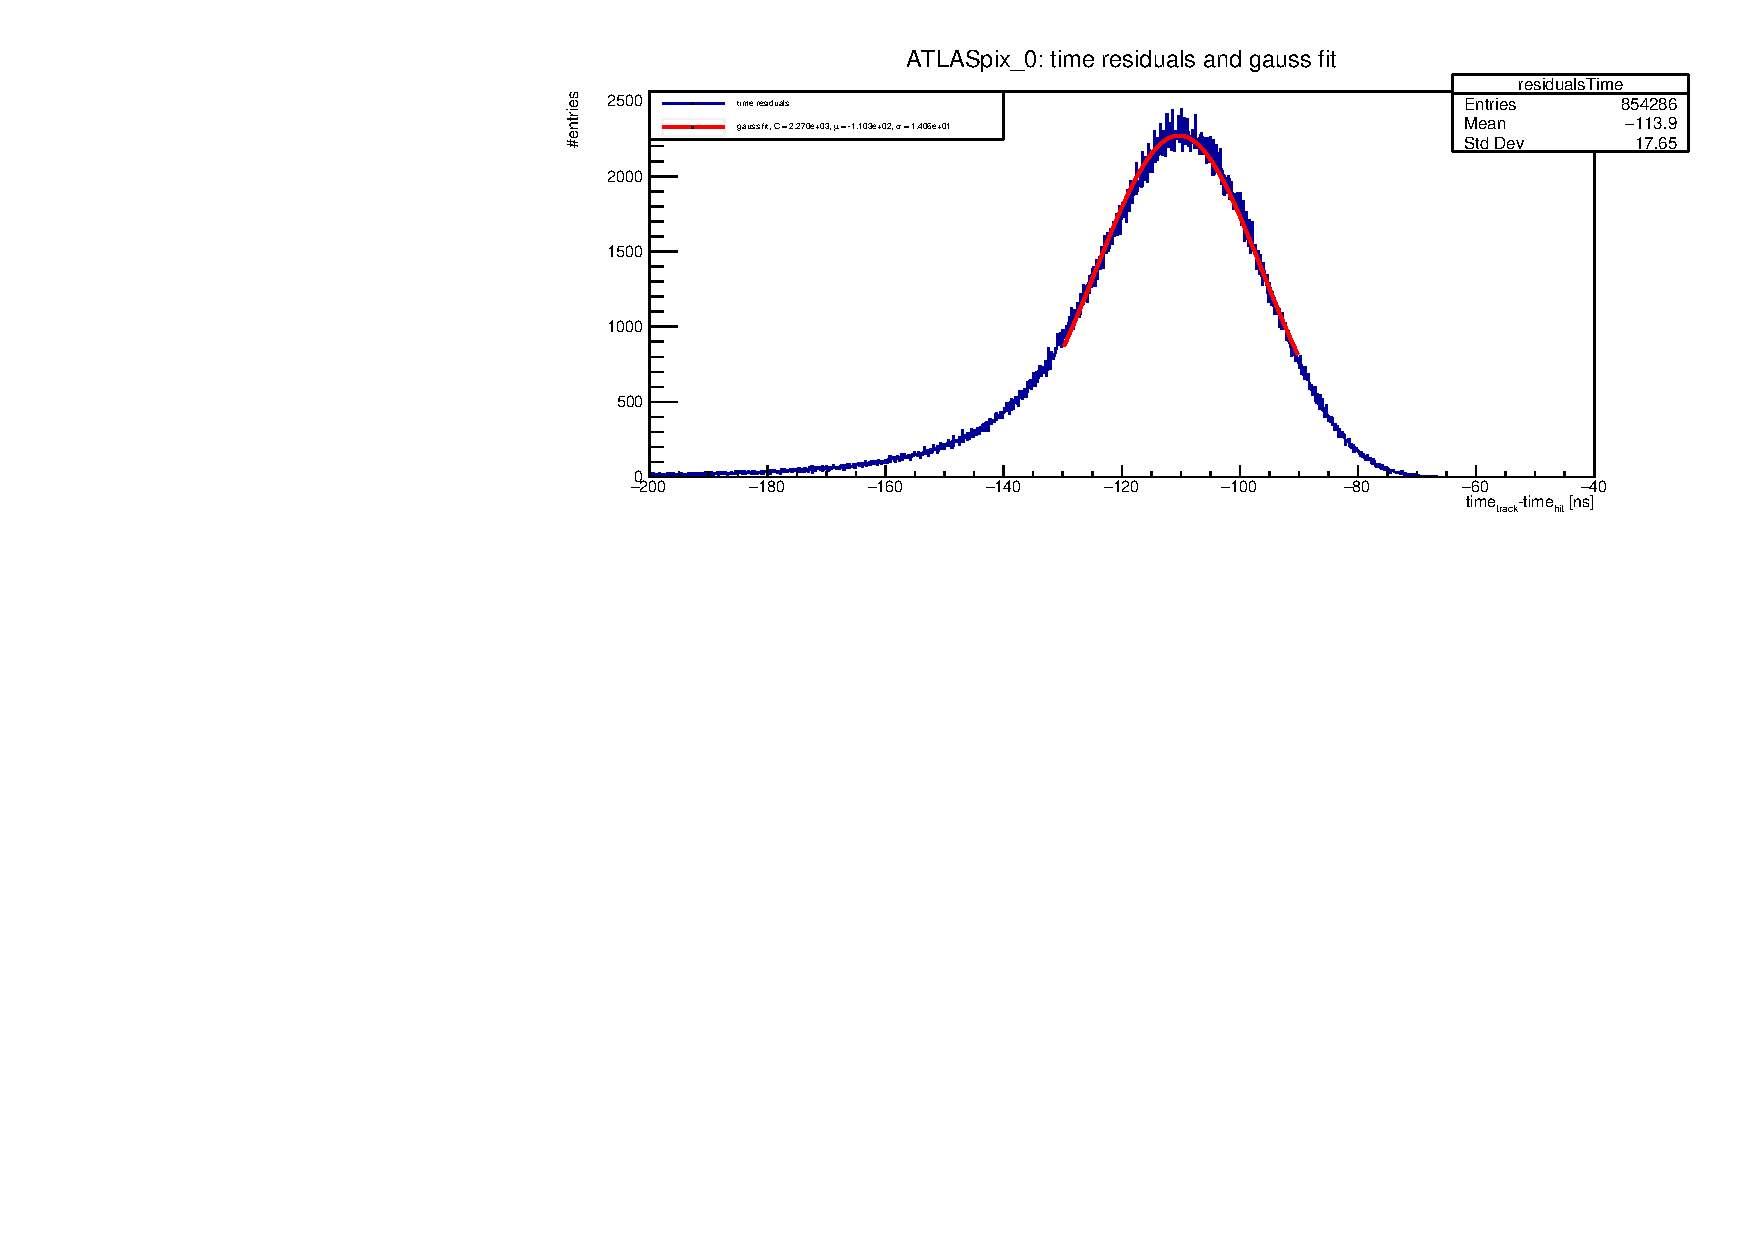
\includegraphics[width=\linewidth]{10_residuals_time.pdf}
  \caption{Time residual distribution}
  \label{fig:time_residuals}
\end{figure}

After correcting our data for the timewalk effect, we repeated the analysis and received a time residual distribution cleared for the timewalk effect, which lacks the overshoot of low time residuals characteristic for the effect (see Fig. \ref{fig:time_residuals_corr}). After this correction, we achieved an improved time resolution

\begin{equation}
  \Delta t = \SI{11.00}{\nano\second}
\end{equation}

\begin{figure}
  \centering
  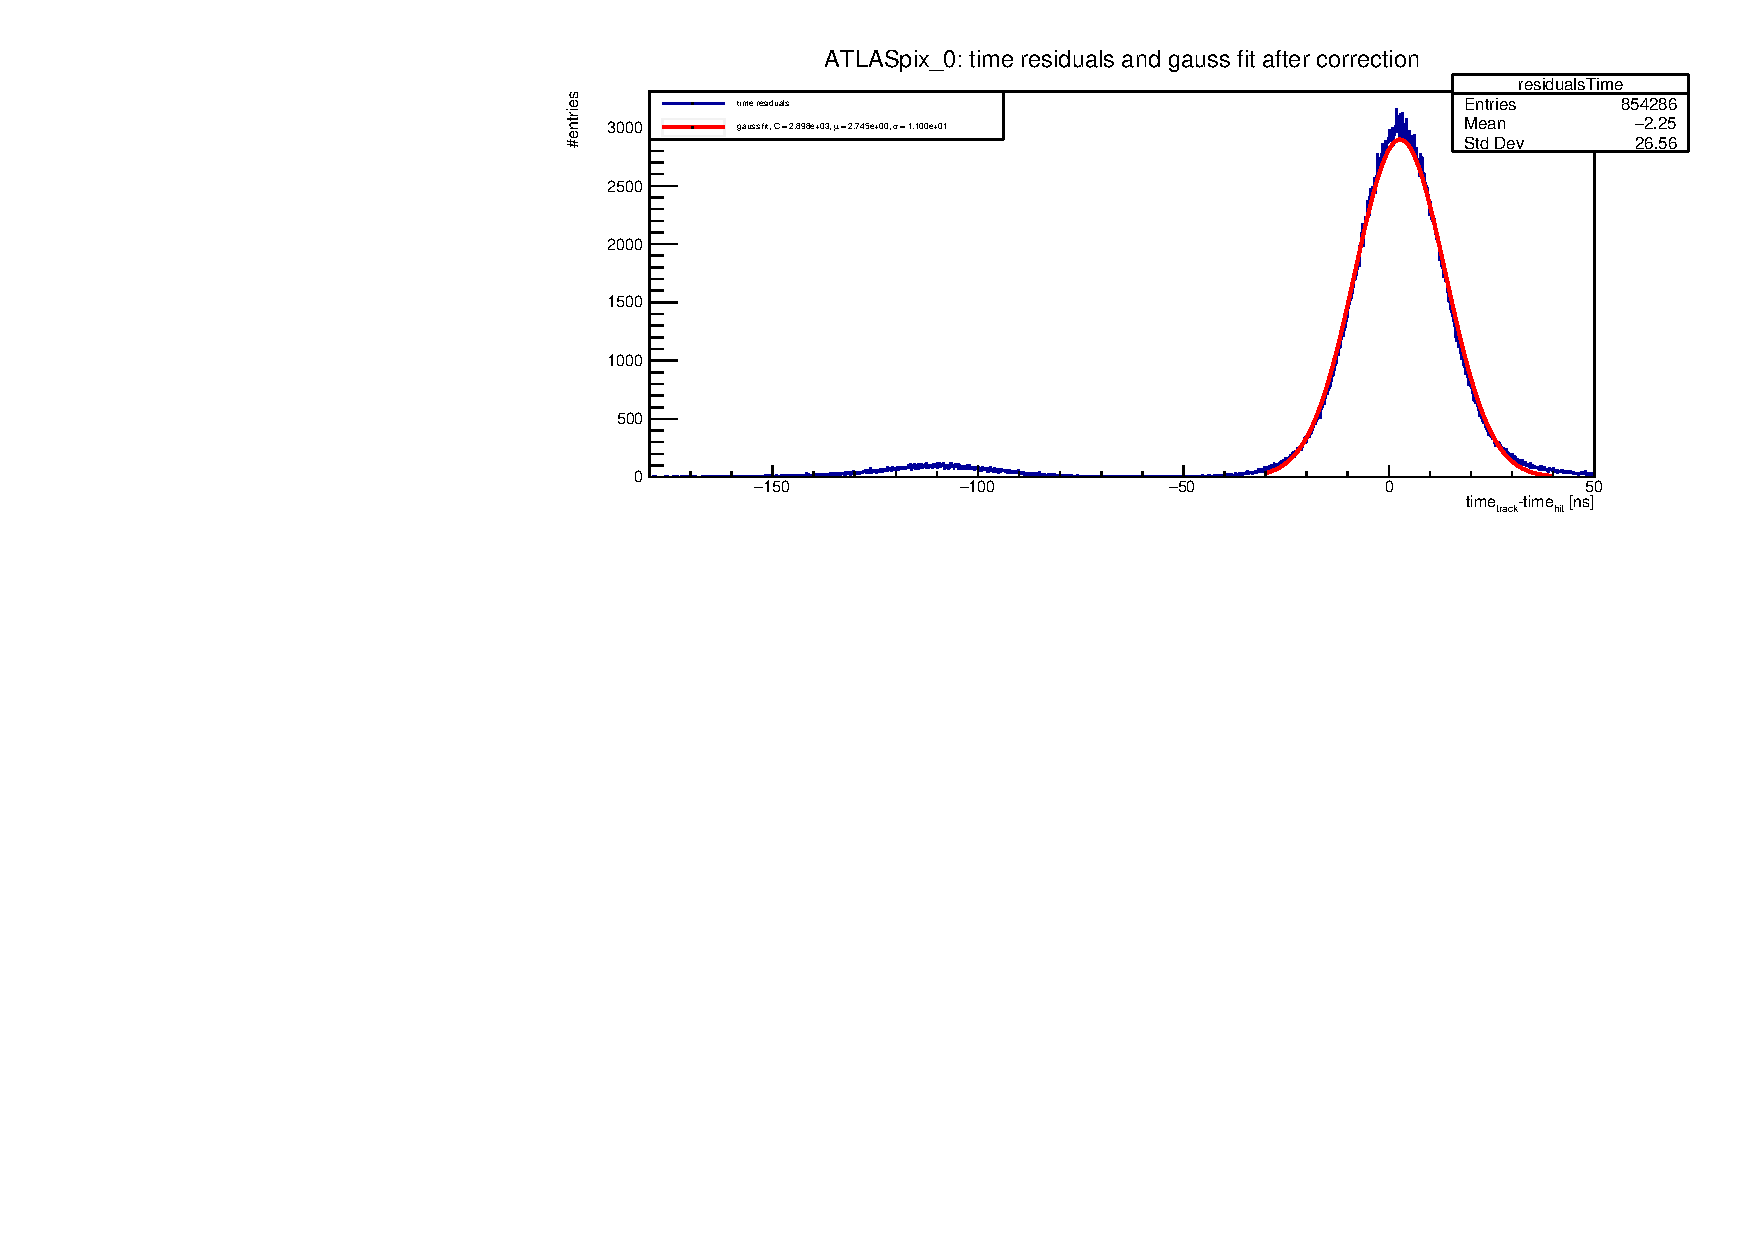
\includegraphics[width=\linewidth]{11_residuals_time_time_correction.pdf}
  \caption{Time residual distribution corrected for timewalk}
  \label{fig:time_residuals_corr}
\end{figure}

By comparing the reference telescope and the \atlaspix, the efficiency of each pixel was determined. That yielded the efficiency map shown in Fig. \ref{fig:efficiency_map}. As the \atlaspix is larger than the reference telescope, data is not available for all pixel. The pixel for which data is available, achieve a mean efficiency of $\num{0.96}$. 

\begin{figure}
  \centering
  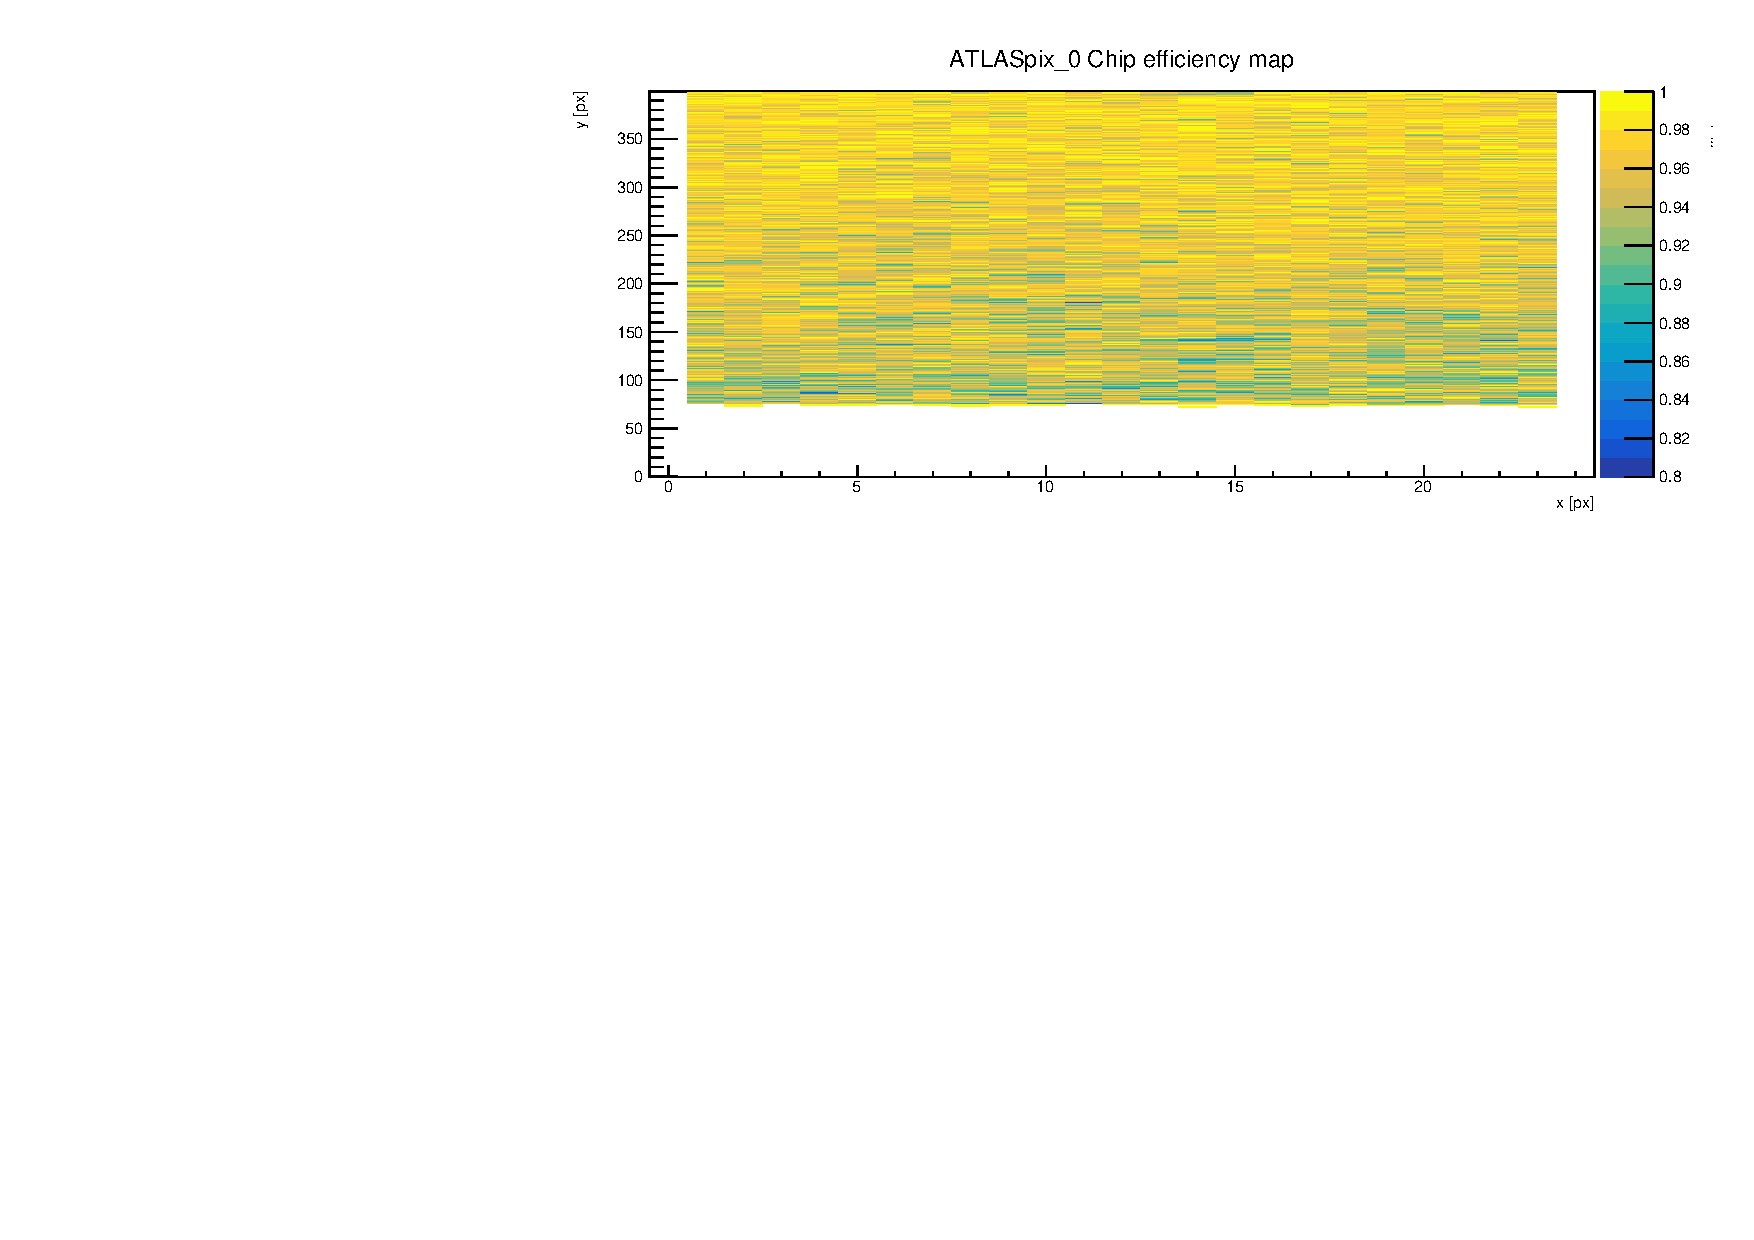
\includegraphics[width=\linewidth]{10_chip_efficiency_map_z_zoom.pdf}
  \caption{Efficiency map for the \atlaspix detector}
  \label{fig:efficiency_map}
\end{figure}

In a last step the influence of the spatial cuts where examined. For this the data analysis was repeated multiple times with varying spatial cuts in x- and y-direction. The result is shown in Fig. \ref{fig:spatial_cuts}. The efficiency seems to vary only slightly spatial cuts larger than the respective pixel dimension, but drops suddenly for spatial cuts smaller than the respective pixel pixel dimension.

\begin{figure}
  \centering
  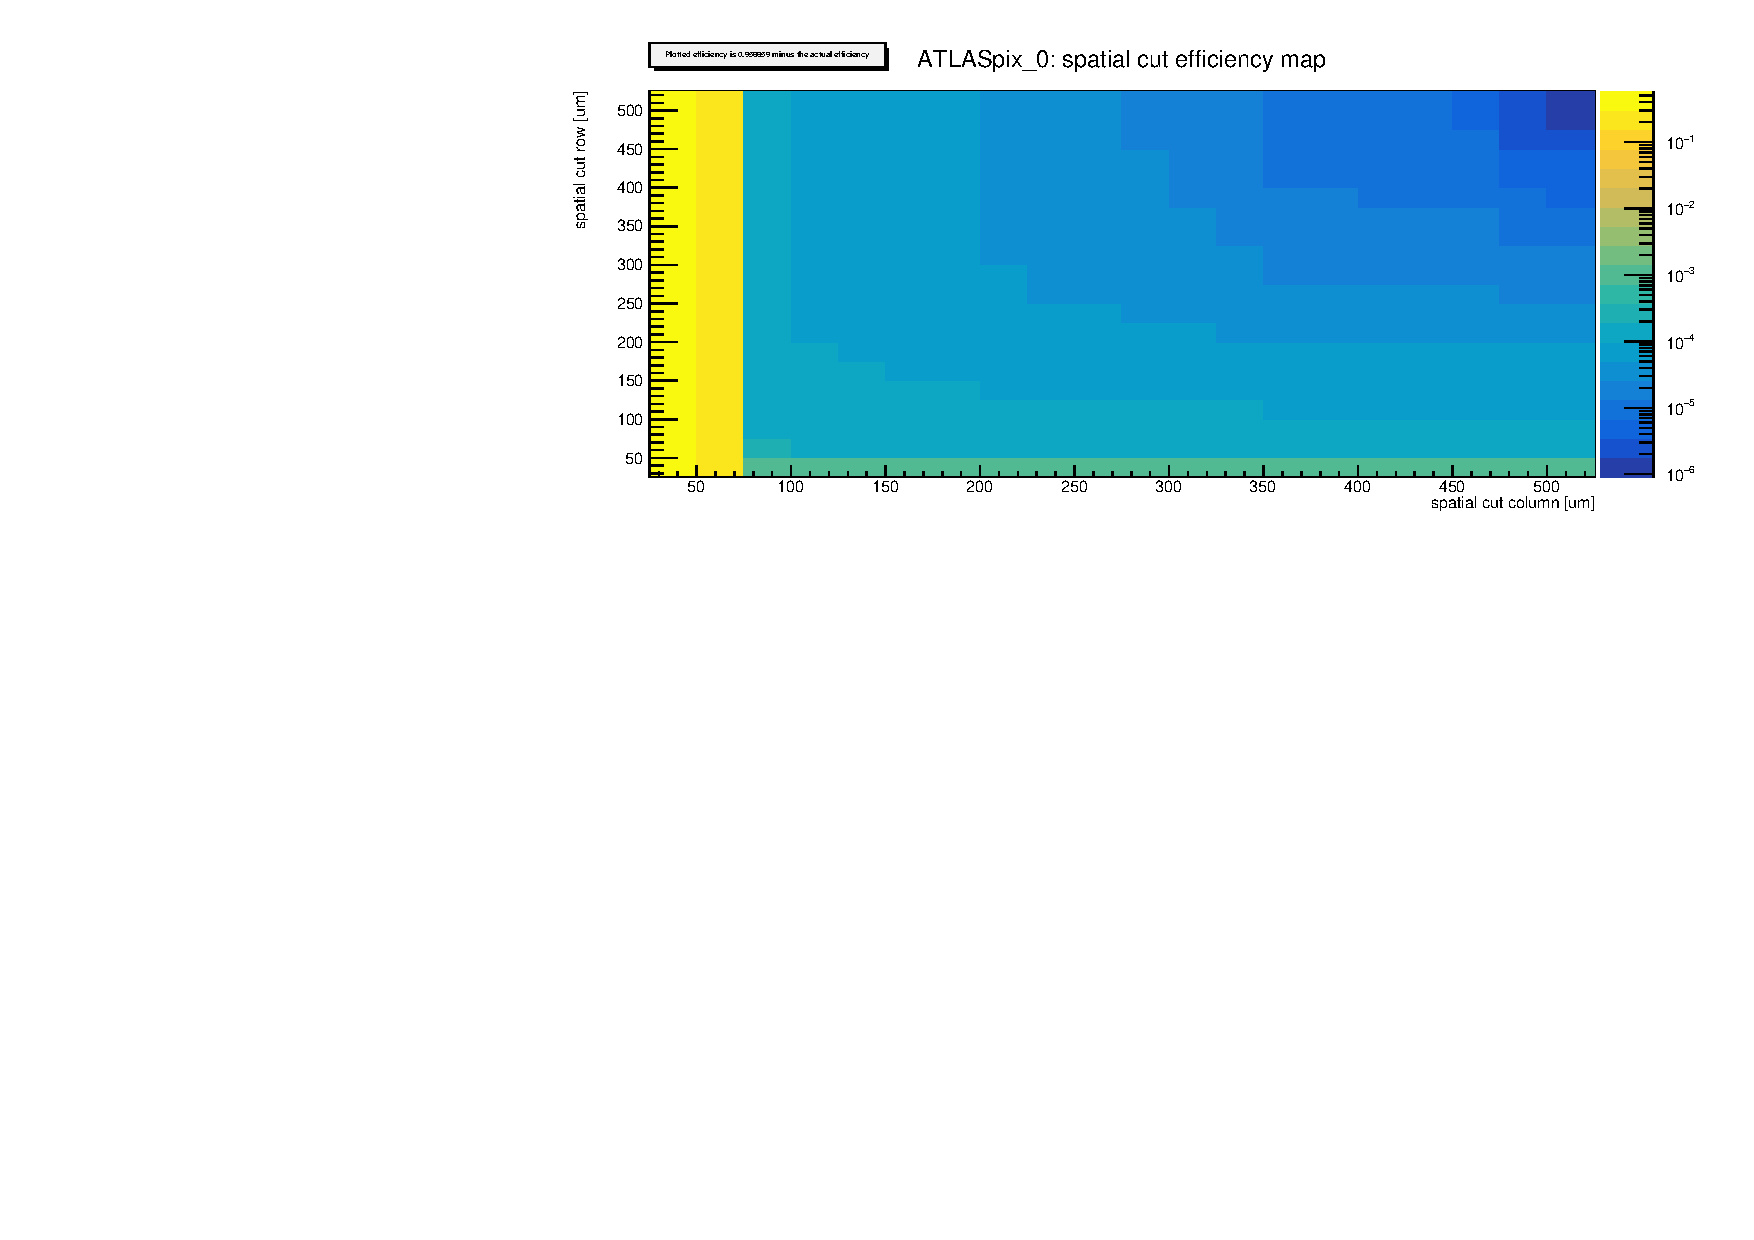
\includegraphics[width=\linewidth]{11_spatial_cut_analysis.pdf}
  \caption{Difference in mean efficiency compared to the previous efficiency in dependence on the spatial cut }
  \label{fig:spatial_cuts}
\end{figure}

\section{Discussion}

The measurement of the time resolution show that the detector is capable to  measure processes on the nanosecond scale. The results could be further improved by optimizing the detectors setting, especially the threshold. The threshold was set at $\SI{950}{\milli\volt}$, which is slightly inefficient. With improved settings even better time resolution are achievable. \cite{} achieved a time resolution of $\SI{8.1}{\nano\second}$ before time walk correction and $\SI{5.9}{\nano\second}$ after timewalk correction. We also see that the timewalk correction helps to improve the resolution significantly and should therefore always be apllied if small timescales are involved.

The efficiency of the chip is in average quite high. But we see a trend of pixels near the edges to have a lower efficiency. That might be caused by an reduced depletion zone in this pixels, which increases the probability of recombination and lowers the efficiency.

We find meanwhile the spatial cut settings to have only a minor influence on the overall efficiency of the sensor as long as the spatial cut is above the respective pixel size. If it is below, single pixels would have to be divided, causing the efficiency to drop as an effective path reconstruction is no longer possible.
\section{Conclusion}

\begin{figure}
  \begin{center}
    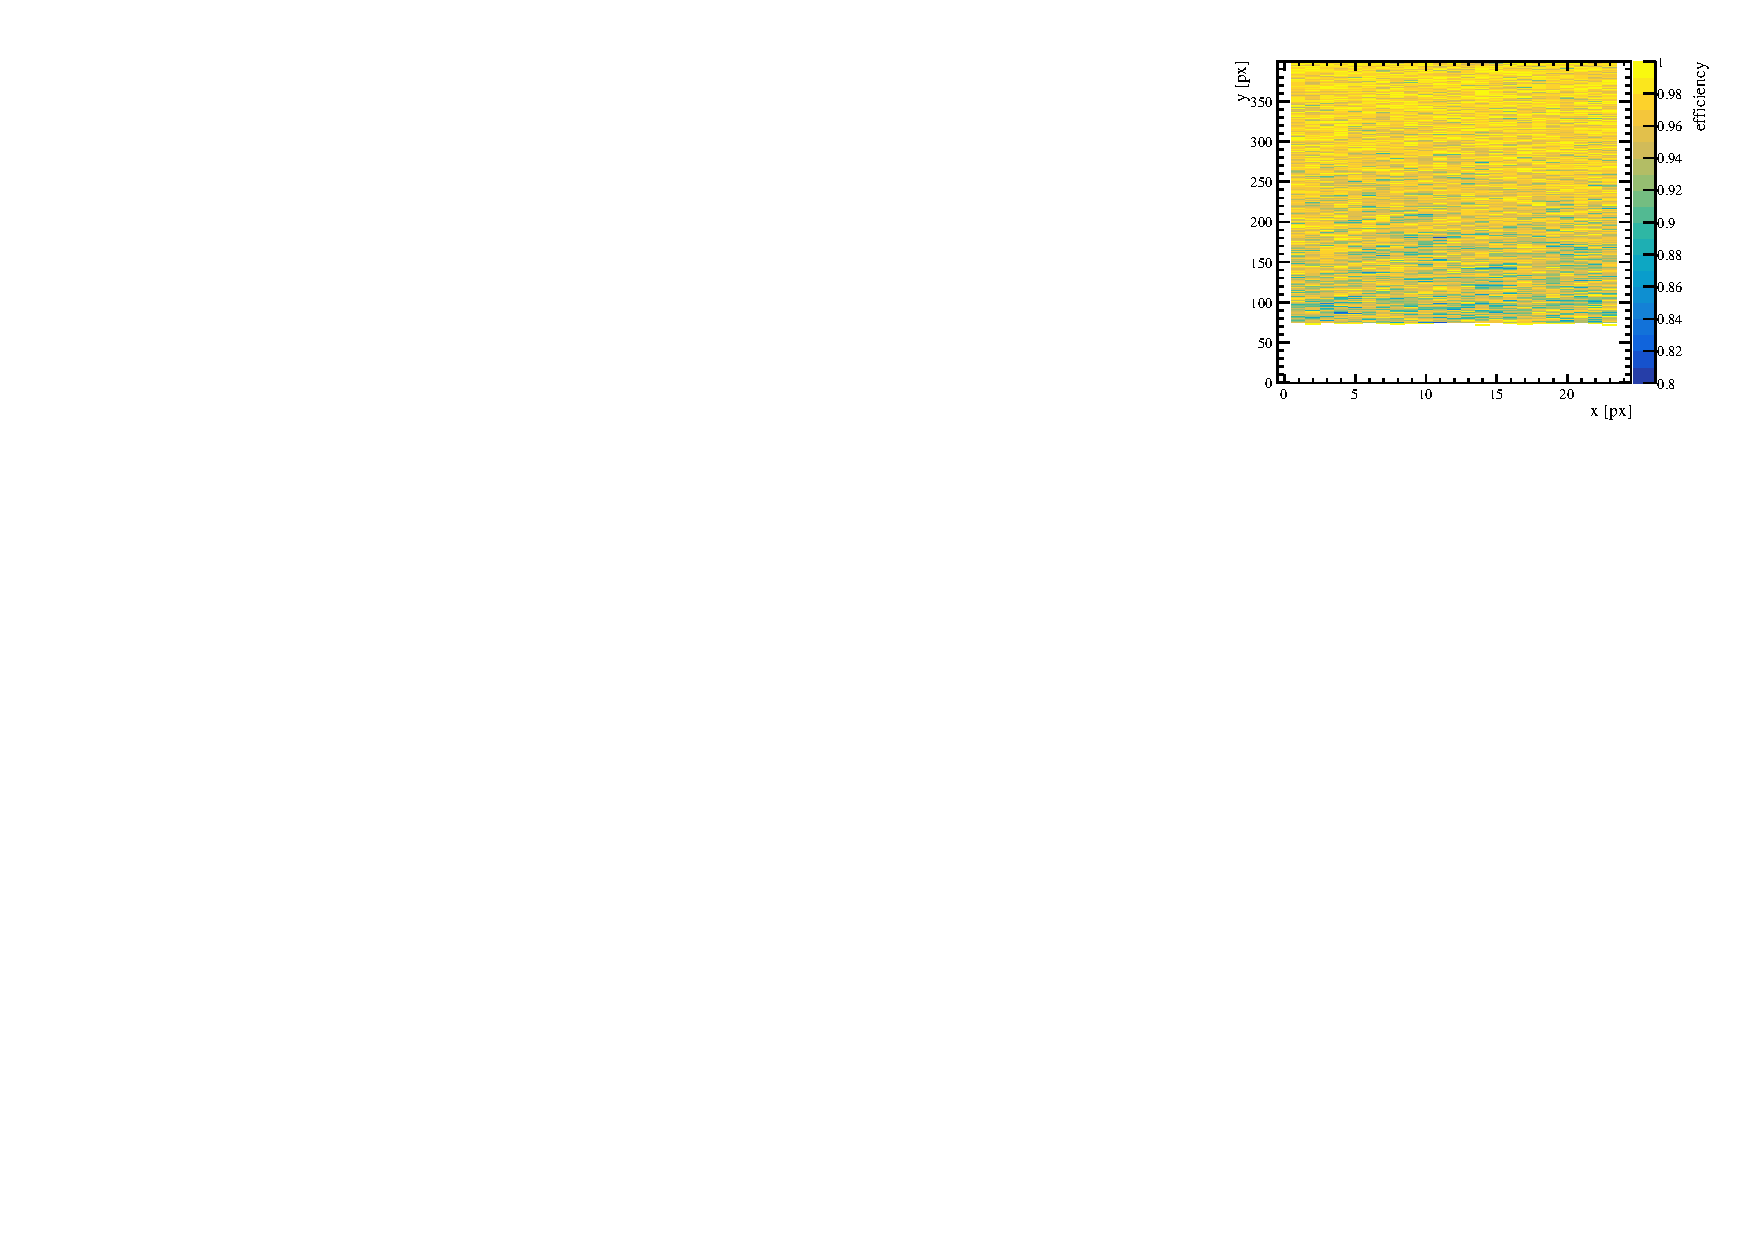
\includegraphics{chip_efficiency}
  \end{center}
  \caption{Chip efficiency map of \atlaspix detector\label{fig:chip_eff}}
\end{figure}

\begin{figure}
  \begin{center}
    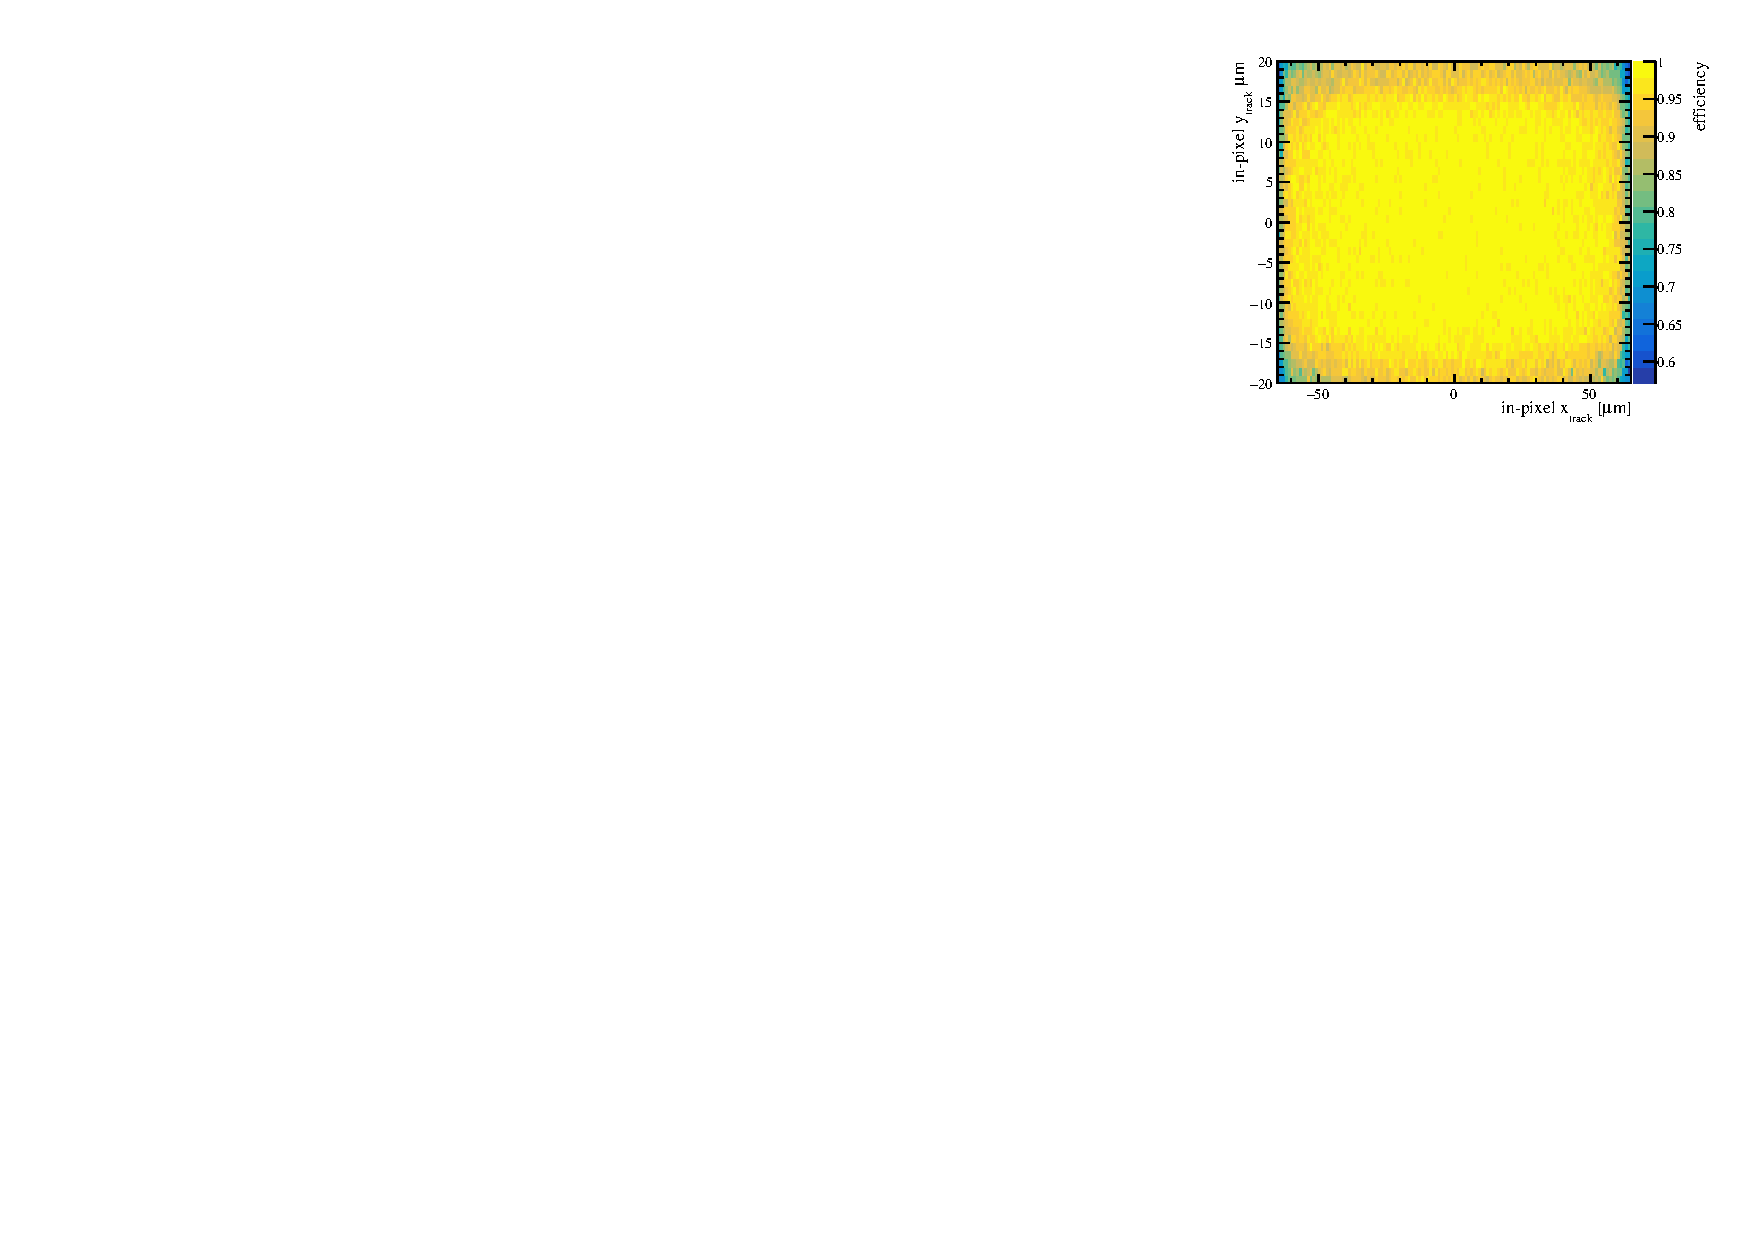
\includegraphics{pixel_efficiency}
  \end{center}
  \caption{Pixel efficiency map of \atlaspix detector\label{fig:pixel_eff}}
\end{figure}

\begin{figure}
  \begin{center}
    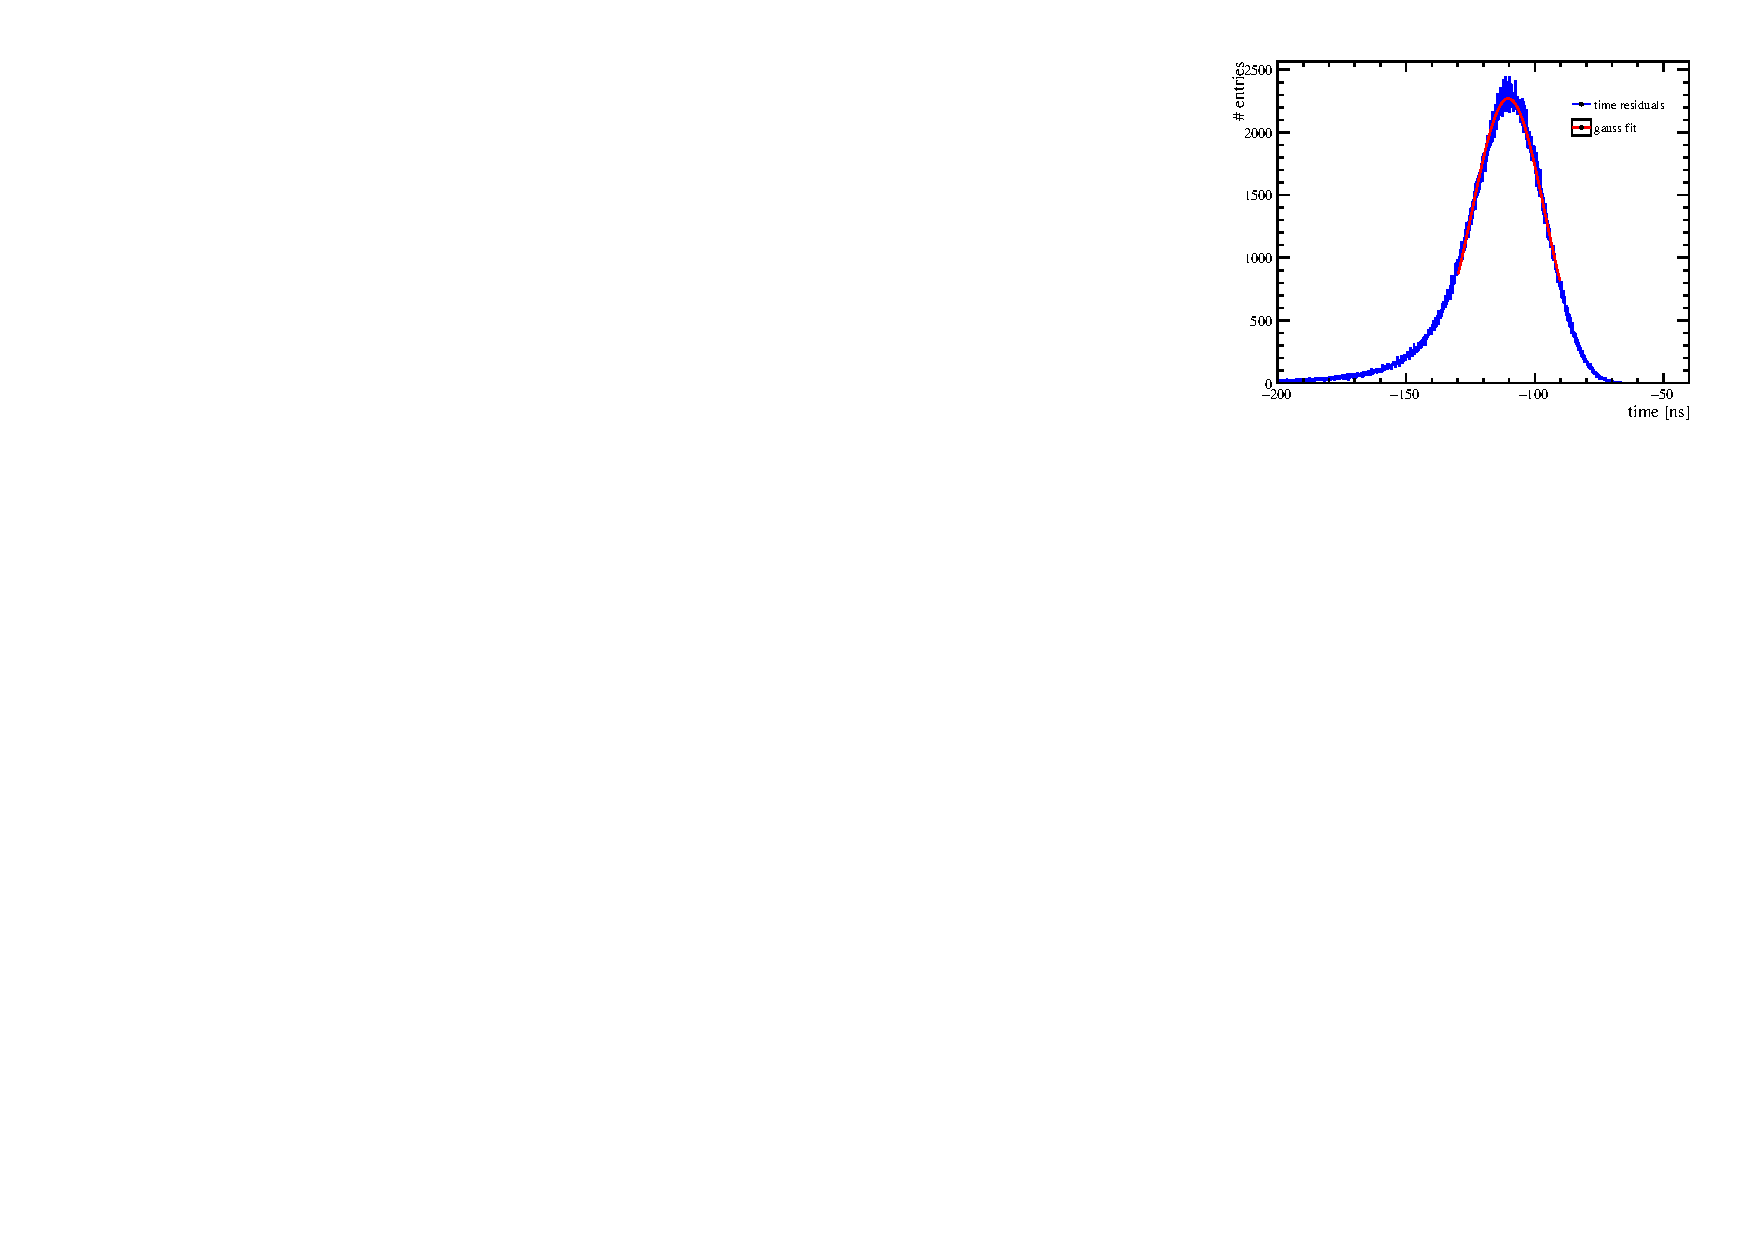
\includegraphics{residuals_time}
  \end{center}
  \caption{Distribution of time residuals for \atlaspix detector\label{fig:time_res}}
\end{figure}

\begin{figure}
  \begin{center}
    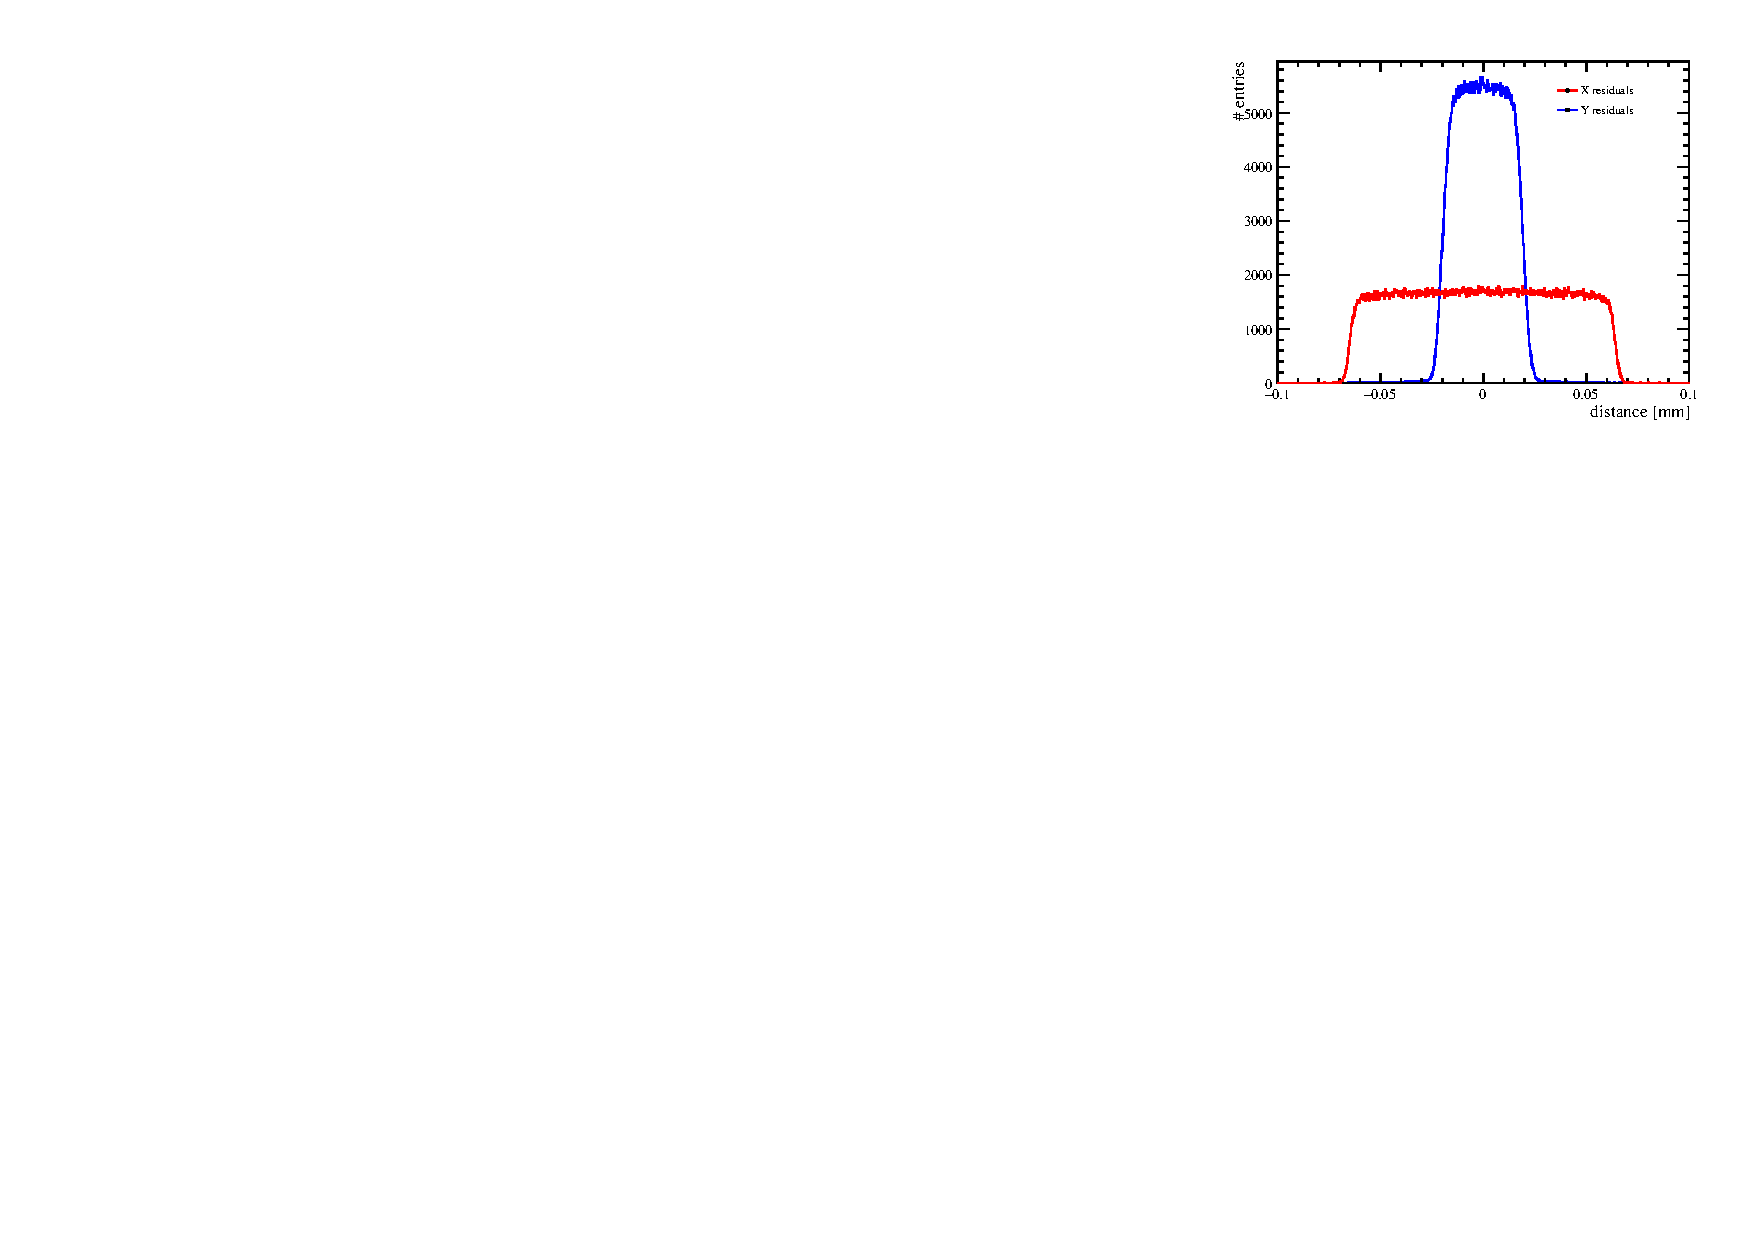
\includegraphics{residuals_x_y}
  \end{center}
  \caption{Distribution $x$ and $y$ time residuals for \atlaspix detector\label{fig:xy_res}}
\end{figure}

\begin{figure}
  \begin{center}
    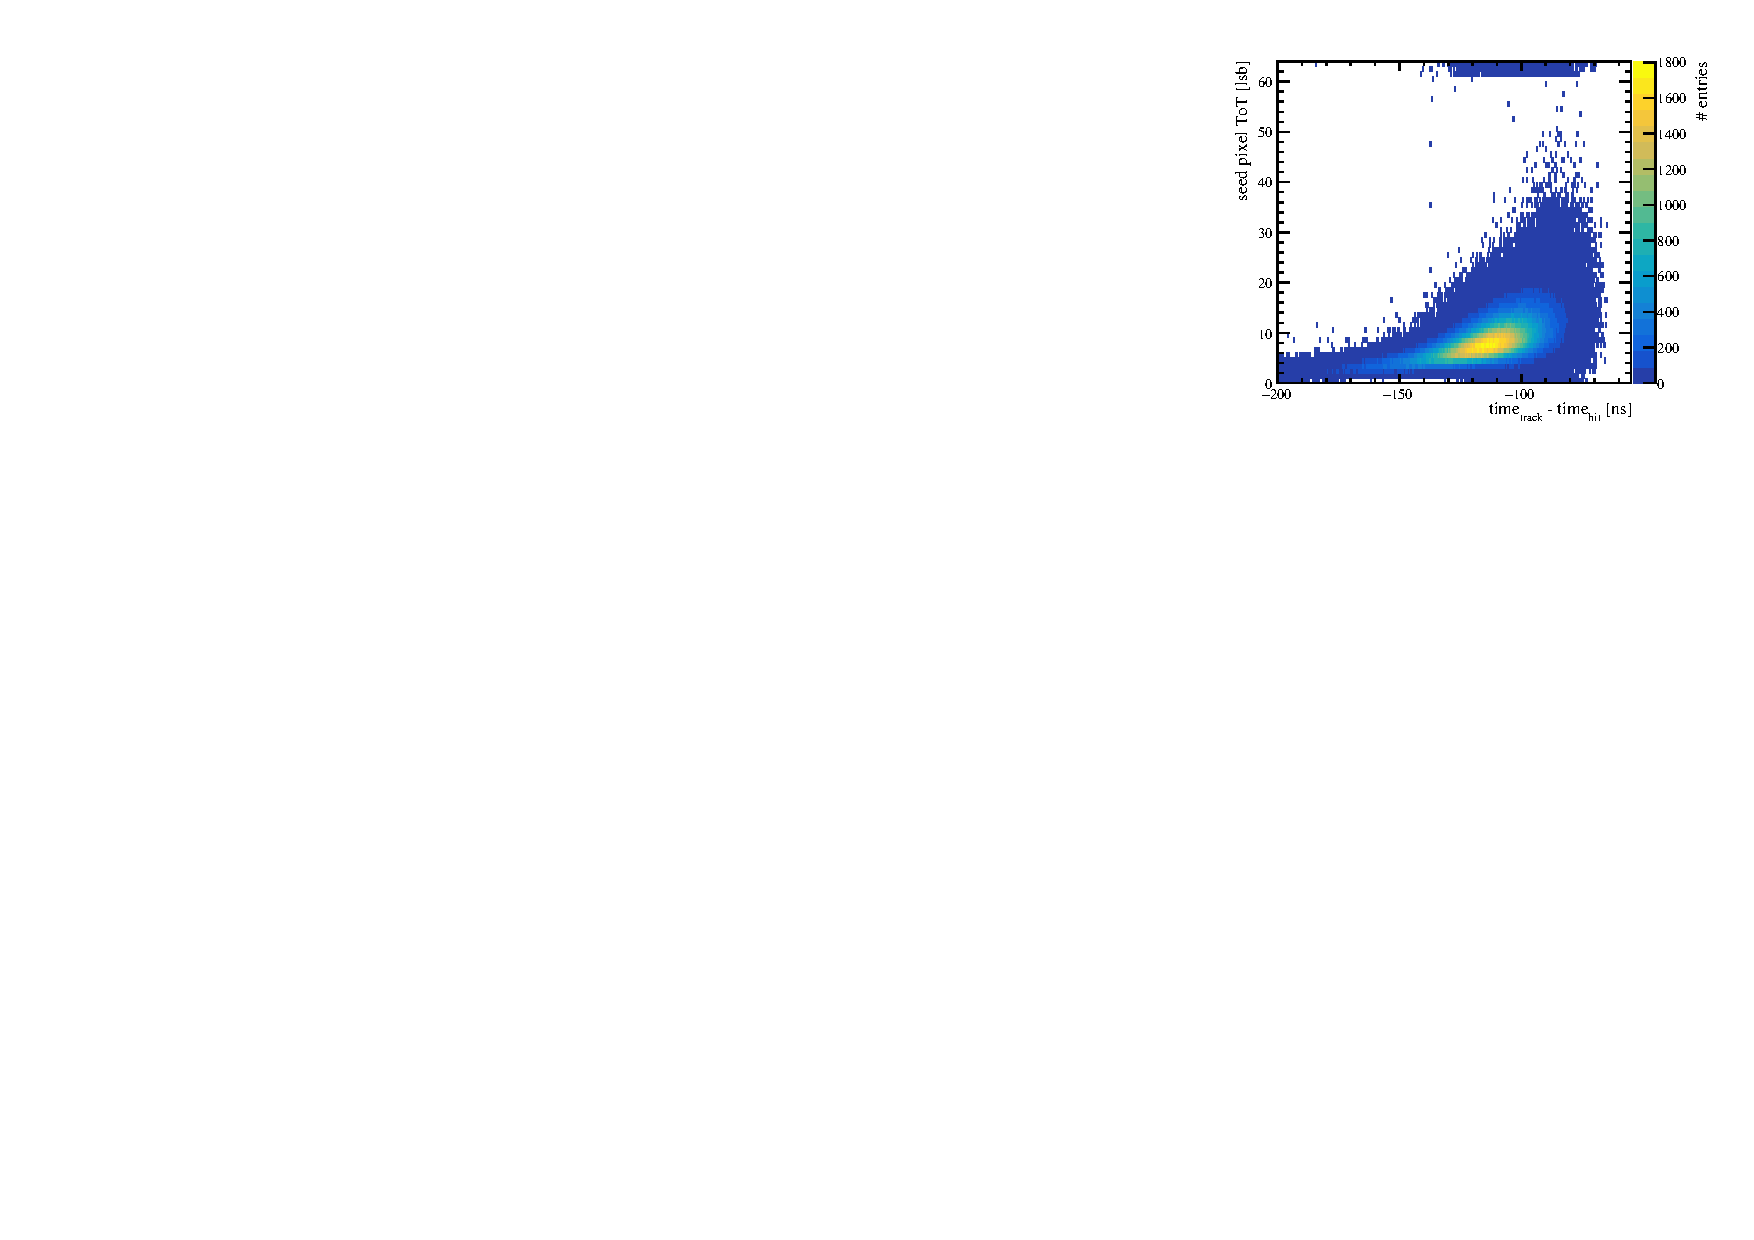
\includegraphics{time_residuals_over_tot}
  \end{center}
  \caption{Time residuals in dependence of seed pixel \tot\label{fig:time_over_tot}}
\end{figure}

\cite{schimassek2020test}
\cite{schoning2020mupix}
\printbibliography
\end{document}
